%
\comment{

--> Talk about how, to support future network bandwidths, the NoC can scale by widening the links

1. Benefit of the NoC-PP modular design is it allows for the easy addition or removal of protocol processing modules
2. This can be used to introduce new protocols or duplicate existing modules to process certain protocols at a higher bandwidth (discussed previously)
3. The 400G use-case of the NoC-PP consists of four duplicates of each protocol's processing module
4. Duplication of a certain protocol can be reduced in order to free up room for other processing modules
5. We would like to explore the impact of removing processing module on performance

}
%

%
\begin{figure*}
\centering
%
        \begin{subfigure}[t]{0.45\textwidth}
        		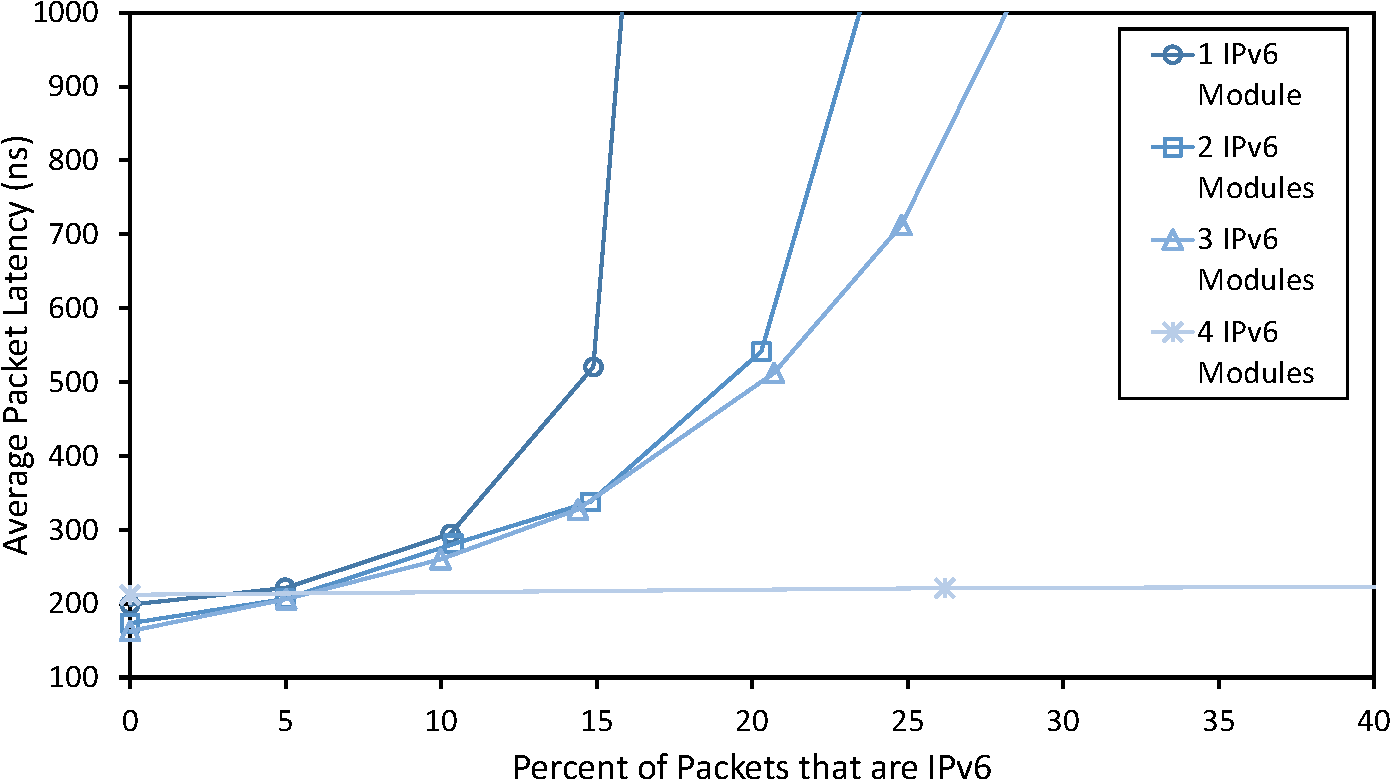
\includegraphics[width=\textwidth]{figs/latency-modules-plot.pdf}
        		\caption{NoC Router Buffer Depth = 10 flits}
        		\label{latency10}
		\end{subfigure}
        \begin{subfigure}[t]{0.45\textwidth}
        		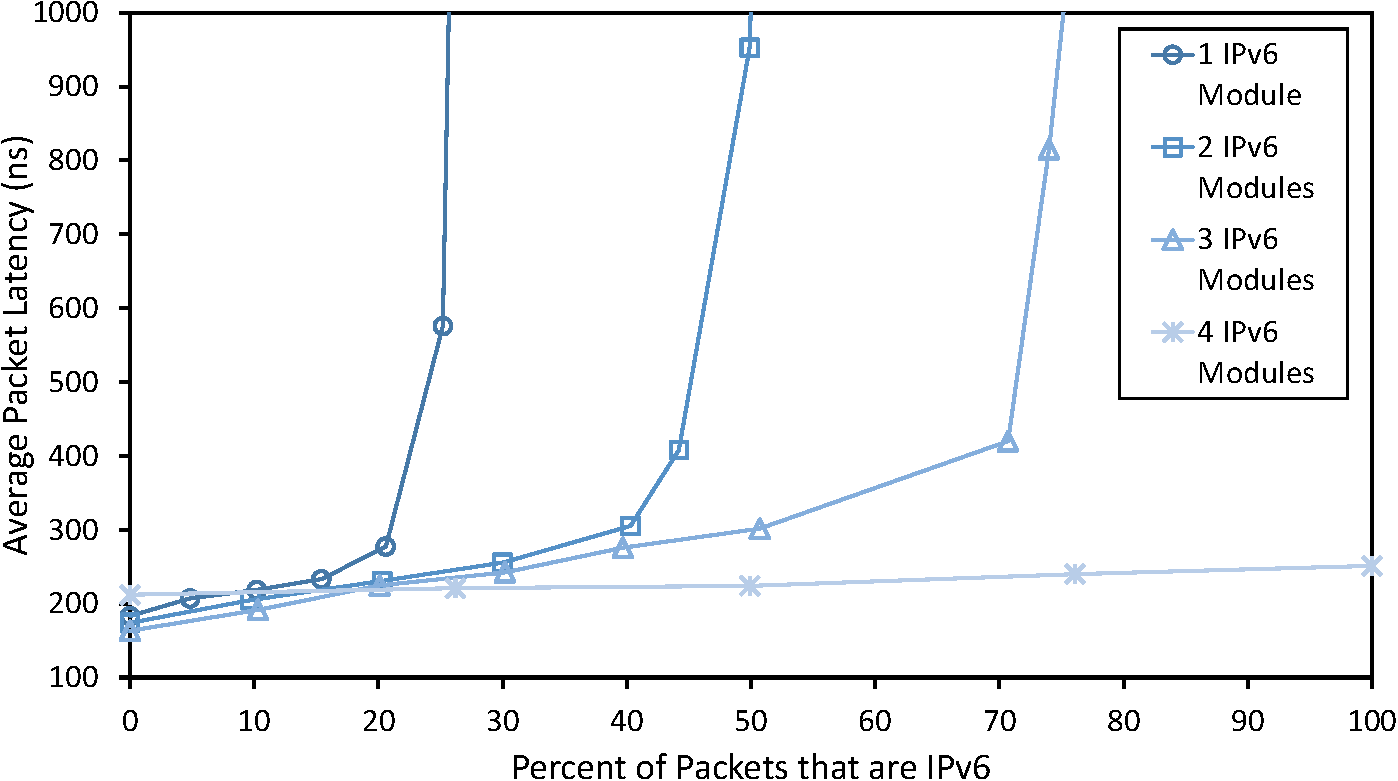
\includegraphics[width=\textwidth]{figs/latency-modules-plot2.pdf}
        		\caption{NoC Router Buffer Depth = 64 flits}
        		\label{latency64}
		\end{subfigure}
\caption{Average packet latency through the NoC-PP design as a function of percentage of total traffic using IPv6, for four different degrees of IPv6 module duplication. Four IPv6 modules (each running at 100G) is sufficient to fully support any rate of IPv6 traffic running at 400G.}
\label{latency-modules}
\end{figure*}
%

%
\begin{figure*}
\centering
%
        \begin{subfigure}[t]{0.4\textwidth}
        		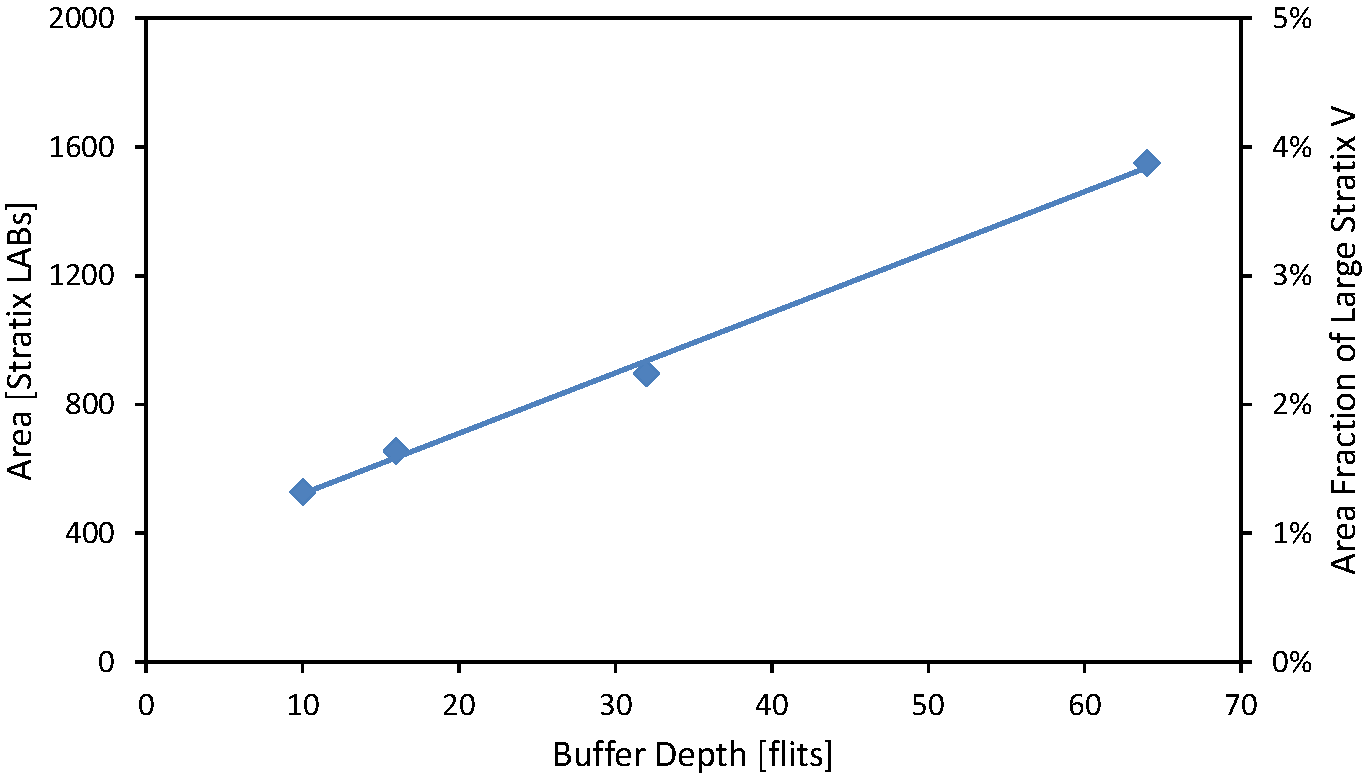
\includegraphics[width=\textwidth]{figs/buffer-depth.pdf}
        		\caption{Embedded NoC Area Scaling with Buffer Depth}
        		\label{buffer-depth}
		\end{subfigure}
        \begin{subfigure}[t]{0.4\textwidth}
        		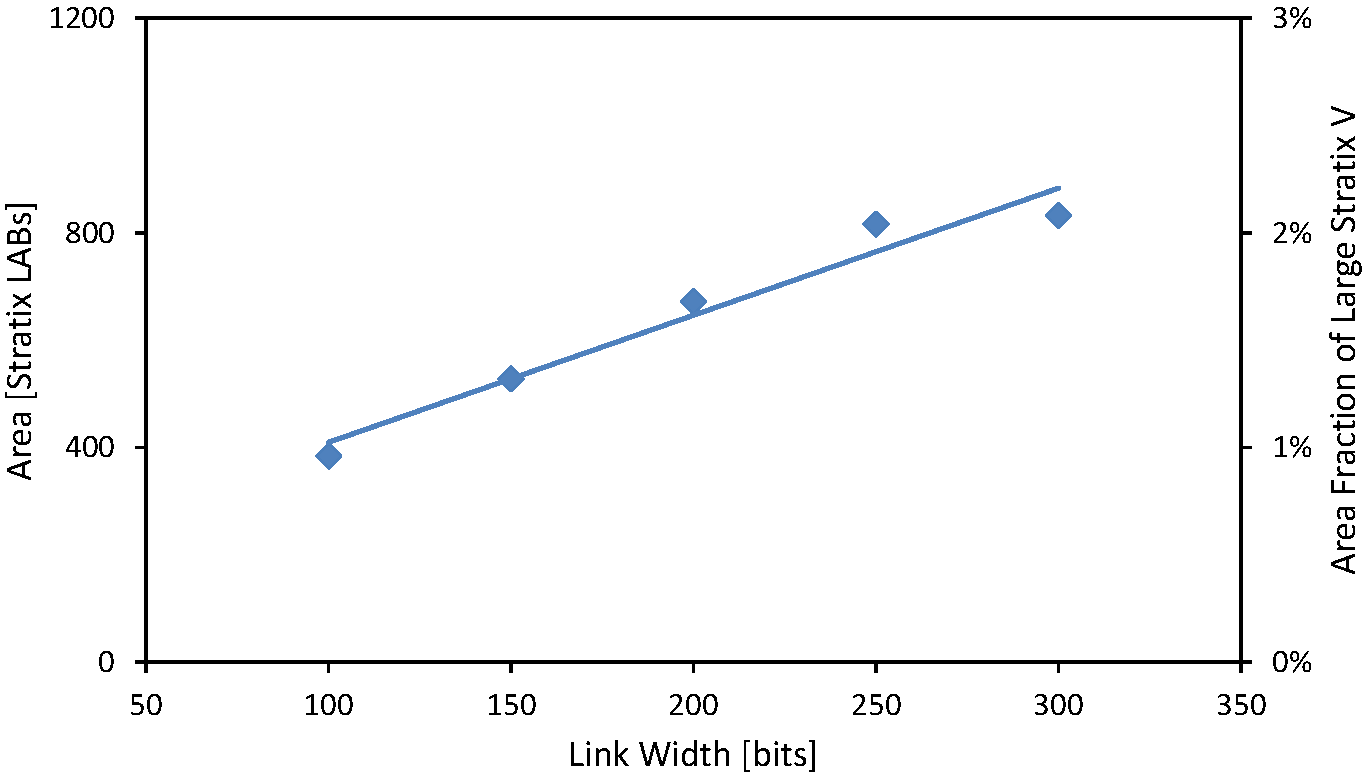
\includegraphics[width=\textwidth]{figs/link-width.pdf}
        		\caption{Embedded NoC Area Scaling with Link Width}
        		\label{link-width}
		\end{subfigure}
\caption{Embedded NoC chip area, measured in equivalent Stratix LABs and fraction of a Stratix V-GS, scaling with buffer depth and link width~\cite{noc-designer}. Figure~\ref{buffer-depth} plots buffer depth with a fixed link width of 150 bits, while Figure~\ref{link-width} plots link width with a fixed buffer depth of 10 flits.}
\label{noc-area}
\end{figure*}
%

The highly modular design of NoC-PP allows for the easy addition and removal of protocol processing modules.
This flexibility can be used to introduce new network protocols, modify protocol processing modules, and duplicate existing protocol modules in order to support higher bandwidths.
The TcpIp4Ip6-Processor design example duplicates each 100G processing module four and eight times in order to fully support 400G and 800G processing, respectively, for each protocol.
Depending on the application, full duplication of each processing module may not be necessary.
It is possible, for example, that a low percentage of the traffic seen by the packet processor uses IPv6\footnote{As of July 2015, Google measures that only $\sim$7\% of accesses to their website are through IPv6~\cite{google_ipv6}.}.
The designer therefore has the flexibility to reduce the number of IPv6 processing modules in order to free up chip area for other modules.

To assess the impact of module duplication on performance, we use \textbf{\texttt{RTL2Booksim}} to simulate the design with varied degrees of duplication of the IPv6 processing module, swept across percentage of the total traffic that is IPv6.
A bursty, 400G traffic pattern is used to emulate real Internet traffic, with packet payload size set to be 512 bytes.
The design is first simulated using a NoC consisting of the same parameters (link width, mesh radix, router buffer depth) as those chosen in previous work~\cite{abdelfattah2015take}.
Figure~\ref{latency10} illustrates the results.
The ``knee'' in each curve indicates the maximum percentage of IPv6 that can be supported at 400G; after this point, the NoC saturates, causing the source to be frequently backpressured.

%\figvs{1}{latency-modules-plot}{}{Average packet latency through the NoC-PP design as a function of percentage of total traffic using IPv6, for four different degrees of IPv6 module duplication. Four IPv6 modules (each running at 100G) is sufficient to fully support any rate of IPv6 traffic running at 400G.}

Originally, it was expected that the design would be able to support up to a fraction of IPv6 packets equal to the number of IPv6 modules implemented divided by four, given it takes four modules to fully support a 100\% IPv6 packet rate (i.e. 25\% for one IPv6 module, 50\% for two, etc.).
However, we see in Figure~\ref{latency10} that the NoC saturates at a much earlier point in each curve.
This can be attributed to the fact that the NoC is not an entirely non-blocking crossbar; packets compete for resources and when one does not receive access to its desired link, it must be held in buffers within the NoC.
In this case, the NoC routers have buffers that can hold 10 NoC flits~\cite{abdelfattah2015take}, while each injected packet forms 40 NoC flits.
Thus, when one packet is waiting for a NoC link to become free, it must be stored in four buffers, consequently congesting four downstream routers.
%When there is more of a mixture of IPv6 along with IPv4 packets, there is more switching in the NoC, as some packets are sorted to either an IPv6 or an IPv4 module.
%With more switching comes more conflicting resource requests, causing congestion to occur.
In the case when four IPv6 modules are implemented, each injection point has its own IPv6 module for its IPv6 packets.
Thus, there is no competition for resources in the NoC.
As soon as there is a mismatch in number of injection points and number of IPv6 modules, packets may compete for resources when two are sent to one IPv6 module at the same time.

One way to mitigate this congestion is to offload the packet payload to external memory until the packet is ready to be sent out, thereby reducing the amount of NoC buffer space consumed by a packet during processing.
This is briefly discussed in Section~\ref{sec:ddr}.
Another method is to increase the buffer depth in the NoC routers.
The impact of buffer size on NoC performance has been studied extensively in previous work~\cite{coenen2006buffer}.
In our application, if a router's buffer could hold an entire packet, rather than just a quarter, it would prevent downstream routers from becoming congested as well.
We test this theory by adjusting the simulated NoC buffer size to 64 flits, rather than 10.
As can be seen in Figure~\ref{latency64}, increasing the buffer size mitigates the NoC's blocking nature, allowing it to saturate according to the availability of IPv6 processing bandwidth in the design.

\vspace{-0.1cm}

The impact of increasing the buffer size of the NoC on its hardware cost is illustrated in Figure~\ref{noc-area}.
Increasing NoC buffer size allows the NoC-crossbar to provide more switching capability for larger packets at a moderate hardware cost.
Figure~\ref{noc-area} also shows the cost of increasing the NoC's inter-router links, which can be used to scale the NoC-crossbar to serve more network bandwidth.
Both of these scaling techniques require architectural changes to an embedded NoC.
Thus, it is crucial that a manufacturer of a NoC-enhanced FPGA appropriately provisions the NoC to serve potential applications.
%We hope our research in this paper and in previous work serves useful for this purpose.
By looking at important FPGA networking applications such as switching~\cite{bitar2014efficient,abdelfattah2015take} and packet processing, we hope to better guide the architectural choices of an embedded NoC.

\vspace{-0.1cm}

Overall, we see that the flexibility that NoC-PP provides to support reprogrammability for network evolution surpasses that of any conceivable ASIC-based packet processor.
NoC-PP is only limited by the amount of resources available on the entire FPGA.
Unlike the RMT design, NoC-PP is not limited by the table sizes and action set established upon chip fabrication.
New actions and match field values can be reprogrammed into new or existing processing modules at any time.
Modules can be modified, replaced and even duplicated by reconfiguring the FPGA fabric.
Not only does NoC-PP manage to exceed the flexibility of the ASIC-based RMT, but it also matches and surpasses RMT's supported bandwidth of 640G.



